\documentclass[10pt,twocolumn]{article}
\usepackage[a4paper,top=20mm,bottom=22mm,left=15mm,right=15mm,columnsep=6mm]{geometry}
\usepackage{amsmath,amssymb,amsfonts}
\usepackage{graphicx}
\usepackage{xcolor}
\usepackage{booktabs}
\usepackage{multirow}
\usepackage{url}
\usepackage[hidelinks]{hyperref}
\usepackage{cite}
\usepackage{caption}
\usepackage{enumitem}
\usepackage{titlesec}

\graphicspath{{figures/}}
\titleformat{\section}{\large\bfseries}{\Roman{section}.}{0.5em}{\MakeUppercase}
\titleformat{\subsection}{\normalsize\itshape}{\Alph{subsection}.}{0.5em}{}
\renewcommand{\thesection}{\Roman{section}}
\renewcommand{\thesubsection}{\Alph{subsection}}
\setlength{\parindent}{1.0em}
\setlength{\parskip}{0pt}

\DeclareMathOperator*{\argmin}{arg\,min}
\newcommand{\R}{\mathbb{R}}
\newcommand{\norm}[1]{\left\lVert #1 \right\rVert}
\newcommand{\misfit}{\Phi}

\title{\bfseries Held-Out Shot Validation for Full-Waveform Inversion Under Modeling Mismatch:
A Marmousi2 Cross-Grid Study}
\author{Anonymous Submission\\
\small\itshape Author identities withheld during peer review}
\date{}

\begin{document}
\twocolumn[\maketitle\begin{@twocolumnfalse}
\begin{abstract}\small
Full-waveform inversion (FWI) is usually controlled by training-data
misfit, but this criterion can become misleading when the inversion
operator differs from the operator that generated the data. We study a
controlled cross-grid Marmousi2 setting in which observed shot gathers are
generated on a fine grid and inverted on a coarser grid after scalar
shot-wise amplitude calibration. The setup preserves known ground truth
for diagnosis while introducing realistic phase and discretization
mismatch. We propose a held-out shot validation rule for selecting the
continuation depth of frequency-domain FWI: after a low-to-high frequency
warmup, last-band L-BFGS-B continuation is run in short chunks, and the
model with minimum validation-shot misfit is selected. The rule is a
model-selection layer around a conventional adjoint FWI solver rather than
a new wave solver or neural parameterization. On the primary Marmousi2
crop, validation selection stops at chunk 2, reducing RMSE from
181.61 to 179.76 m/s relative to the final continued model, increasing
SSIM from 0.5187 to 0.5241, and improving edge correlation from 0.2556 to
0.2648 while the training misfit continues to decrease. Across three
independent shot splits on the same crop, validation-selected models
outperform final continuation in RMSE, SSIM, $R^2$, and edge correlation.
The same rule remains beneficial at 20 dB and 10 dB additive noise. A
second crop shows a more limited pattern: overfitting appears later and
not in every split, but validation selection avoids degradation in two of
three long-continuation splits. These results support held-out shot
validation as a practical stopping rule for FWI under modeling mismatch,
with a deliberately limited claim: it detects and controls continuation
overfitting when validation data expose it, but it is not a universal
substitute for improved physics, acquisition design, or stronger priors.
\end{abstract}
\vspace{0.75em}
\noindent\textbf{Keywords:} full-waveform inversion; Marmousi2; validation
stopping; modeling mismatch; L-BFGS-B; cross-grid inversion; seismic
imaging.
\vspace{1.0em}
\end{@twocolumnfalse}]

% =====================================================================
\section{Introduction}
% =====================================================================
Full-waveform inversion (FWI) estimates subsurface velocity by minimizing
the mismatch between observed and simulated waveforms
\cite{tarantola1984inversion,virieux2009overview}. The method is
appealing because it uses the full recorded waveform, but the optimization
is nonconvex, sensitive to the starting model, and affected by cycle
skipping, incomplete illumination, and model error
\cite{pratt1999seismic,bunks1995multiscale,vanleeuwen2013mitigating}.
Limited-memory quasi-Newton methods such as L-BFGS and L-BFGS-B remain
standard numerical workhorses because they provide scalable curvature
information without forming the Hessian explicitly
\cite{nocedal1980updating,liu1989limited,byrd1995limited}. In practice,
however, lower training misfit does not always imply a better velocity
model. This is especially true when the forward operator used for
inversion is only an approximation of the process that generated the data.
As FWI implementations become easier to modify through modern numerical
and automatic-differentiation workflows \cite{zhu2021integrating}, the
need for validation designs that detect operator-specific overfitting
becomes more important rather than less important.

Modeling mismatch is unavoidable in seismic inversion. Field-data
applications face source uncertainty, attenuation, elastic effects,
anisotropy, unknown acquisition details, and numerical discretization
differences. Even synthetic studies can hide mismatch if the same grid,
time step, boundary treatment, and forward code are used to generate and
invert the data. Such inverse crimes make algorithmic progress difficult
to evaluate. A useful intermediate test is therefore to keep the problem
synthetic and measurable while deliberately separating the data-generation
operator from the inversion operator.

This paper studies a compact but controlled version of that idea. We
generate observed data from a fine-grid Marmousi2 P-wave velocity subset
\cite{versteeg1994marmousi,martin2006marmousi2}, then invert on a
coarser grid using the same acoustic solver family. Fine-grid data are
resampled to the coarse receiver locations and calibrated shot by shot
against the coarse response at the initial model. This calibration removes
the dominant amplitude scale mismatch while preserving phase and
discretization mismatch. The true coarse model is retained only for
diagnostic metrics; it is not used by the proposed stopping rule.

Our contribution is a validation-controlled continuation rule for FWI
under this controlled mismatch. The rule splits shots into training and
validation sets. Training shots drive the adjoint L-BFGS-B update; held-out
shots are used only to evaluate continuation checkpoints. After a
low-frequency warmup, high-frequency continuation proceeds in short
chunks, and the selected model is the checkpoint with the lowest held-out
shot misfit. This is conceptually close to validation and generalized
cross-validation ideas in inverse problems and statistical model selection
\cite{golub1979generalized,hansen2010discrete}, but here the validation
unit is a physical shot gather rather than a random sample of pixels or
traces.

The claim is intentionally narrow. We do not introduce a new wave solver,
neural parameterization, or regularizer. We also do not claim universal
superiority over continued pixel-domain FWI. Instead, we show that
held-out shot validation provides a reproducible criterion for detecting
and avoiding continuation overfitting when the training objective keeps
decreasing while validation data and true-model metrics degrade.

% =====================================================================
\section{Related Work}
% =====================================================================
\subsection{FWI, Continuation, and Alternative Misfits}
The proposed validation layer sits on top of a long line of waveform
inversion research. Early nonlinear waveform inversion studies established
the feasibility and difficulty of fitting seismic waveforms directly
\cite{gauthier1986twodimensional,mora1987nonlinear,pratt1990crosshole,
pratt1998gaussnewton,pratt1999seismic}. Multiscale frequency strategies
and practical frequency-domain workflows remain central to reducing
cycle-skipping risk
\cite{bunks1995multiscale,sirgue2004efficient,ravaut2004multiscale,
sirgue2010valhall,warner2013anisotropic,virieux2009overview}.
Adjoint-state methods and
PDE-constrained optimization provide the gradient machinery behind these
workflows
\cite{plessix2006review,tromp2005seismic,fichtner2006adjoint,
haber2012effective,metivier2013truncated}, while velocity-analysis and
reflection-inversion perspectives clarify the limits of waveform-only
updates when low-wavenumber information is missing
\cite{symes2008migration,symes2009reflection}.

Several complementary approaches attempt to make FWI less sensitive to
local minima, noise, or modeling error. These include wave-equation
traveltime or skeletonized objectives
\cite{luo1991traveltime,luo1991skeletalized}, robust residual norms
\cite{ha2009huber,brossier2009l1,brossier2010norm}, phase/envelope and
adaptive waveform inversion
\cite{bozdag2011misfit,warner2016adaptive,guasch2019adaptive}, optimal
transport and Wasserstein-type misfits
\cite{engquist2014wasserstein,metivier2016otgji,metivier2016ottle,
yang2018ot}, expanded or relaxed search spaces
\cite{vanleeuwen2013mitigating,vanleeuwen2016penalty}, stochastic source
or data subsampling \cite{vanleeuwen2011stochastic}, and explicit
regularization strategies
\cite{asnaashari2013regularized,esser2018tv}. The present paper is
orthogonal to these methods: it does not replace the objective or
regularizer, but selects among checkpoints produced by a conventional
continuation run. In principle, the same validation criterion could be
wrapped around many of these inversion variants.

\subsection{Validation, Regularization, and Model Mismatch}
The use of validation data for model selection has a long statistical
history
\cite{stone1974cross,allen1974relationship,geisser1975predictive,
stone1977asymptotics,arlot2010survey}. Generalized cross-validation and
related smoothing-parameter criteria were developed for noisy inverse and
regularized estimation problems
\cite{wahba1977practical,craven1978smoothing,golub1979generalized,
wahba1990spline,hansen1992lcurve,hansen1993lcurve,hanke1996heuristic,
reginska1996regularization,kilmer2001choosing,belge2002efficient,
bauer2011comparing}. Iterative stopping can also act as regularization
\cite{prechelt1998early,zhang2005boosting,yao2007early,
raskutti2014early,hardt2016train}, but validation-based stopping can
itself overfit when the validation protocol is not reported carefully
\cite{varma2006bias,cawley2010overfitting}. These caveats motivate our
choice to report the selected checkpoint, the final checkpoint, and
truth-based oracle diagnostics separately.

Classical inverse-problem literature frames these issues more broadly in
terms of ill-posedness, regularization, discrepancy principles, and
statistical uncertainty
\cite{tikhonov1977solutions,morozov1984methods,engl1996regularization,
vogel2002computational,tarantola2005inverse,kaipio2005statistical,
hansen2010discrete,stuart2010bayesian,calvetti2018inverse}. Our
cross-grid setup is also motivated by the inverse-crime and model
discrepancy literature
\cite{kaipio2007inversecrimes,arridge2006approximation,
kennedy2001calibration,brynjarsdottir2014modeldiscrepancy,
lu2014discrepancy,banks2016difference,lieberman2010modelreduction}.
Generating data on a finer grid and inverting on a coarser grid is not a
complete model-discrepancy treatment, but it is a controlled way to avoid
a same-operator synthetic test while retaining known ground truth.

\subsection{Reproducible Computational Geoscience}
The paper also follows the reproducible-computation tradition in
geophysics and scientific computing
\cite{claerbout1992electronic,schwab2000making,buckheit1995wavelab,
donoho2009reproducible,peng2011reproducible,sandve2013tenrules,
wilson2014best,wilson2017good,stodden2016enhancing,
gil2016geosciencepaper,konkol2019geoscience,piccolo2016tools,
hutton2020bmi}. All reported tables and figures are derived from saved
JSON summaries, model checkpoints, and figure-generation scripts. This is
important for a stopping-rule paper because the selected checkpoint,
validation curve, and final model must be auditable rather than chosen
manually after inspecting the truth.

% =====================================================================
\section{FWI With Held-Out Shot Validation}
% =====================================================================
\subsection{Training and Validation Objectives}
Let $v\in\R^{n_z\times n_x}$ denote the velocity model on the inversion
grid. For frequency band $b$ and shot $s$, let $F_{b,s}(v)$ be the
coarse-grid acoustic forward operator and let $\tilde d_{b,s}$ be the
calibrated observed shot gather sampled at coarse receiver locations. For
a set of training shots $\mathcal{T}$, the inversion minimizes
\begin{equation}
  \misfit_{\mathcal{T}}(v)
  = \frac{1}{2}\sum_{b}\sum_{s\in\mathcal{T}}
    \norm{F_{b,s}(v)-\tilde d_{b,s}}_{\Delta t}^{2},
  \label{eq:train}
\end{equation}
where $\norm{x}_{\Delta t}^{2}=\Delta t\sum_i x_i^2$. Gradients are
computed using the discrete adjoint-state method
\cite{plessix2006review,virieux2009overview}.

For held-out shots $\mathcal{V}$, we define
\begin{equation}
  \misfit_{\mathcal{V}}(v)
  = \frac{1}{2}\sum_{b}\sum_{s\in\mathcal{V}}
    \norm{F_{b,s}(v)-\tilde d_{b,s}}_{\Delta t}^{2}.
  \label{eq:validation}
\end{equation}
No gradient is taken through \eqref{eq:validation}. It is used only to
choose among saved continuation checkpoints.

\subsection{Cross-Grid Calibration}
Observed data are generated on a fine grid by a forward operator
$F^f_{b,s}$. The fine shot gather $d^f_{b,s}$ is sampled at receiver
locations corresponding to the coarse grid. A scalar calibration factor is
then estimated from the initial model $v_0$:
\begin{equation}
  \alpha_{b,s}
  = \frac{\langle F_{b,s}(v_0), d^f_{b,s}\rangle}
         {\langle d^f_{b,s}, d^f_{b,s}\rangle},
  \qquad
  \tilde d_{b,s} = \alpha_{b,s} d^f_{b,s}.
  \label{eq:calibration}
\end{equation}
This step is intentionally simple: it corrects first-order amplitude scale
differences without giving the inversion access to the target velocity.
The remaining mismatch comes from grid spacing, time stepping, numerical
dispersion, and phase differences between the fine and coarse operators.

\subsection{Continuation Selection Rule}
The inversion first runs a multiscale warmup over low-to-high Ricker
source frequencies. It then continues on the highest band in fixed-size
optimization chunks. Let $v_{-1}$ be the warmup result and
$v_0,\ldots,v_K$ be the last-band continuation checkpoints. The selected
model is
\begin{equation}
  v_{k^\star},\qquad
  k^\star = \argmin_{k\in\{-1,0,\ldots,K\}}
            \misfit_{\mathcal{V}}(v_k).
  \label{eq:selection}
\end{equation}
The final continued model $v_K$ is reported as a baseline. Oracle models,
defined by the minimum RMSE or maximum SSIM over the checkpoints, are
reported only for analysis because they require the known true model.

% =====================================================================
\section{Experimental Design}
% =====================================================================
\subsection{Marmousi2 Cross-Grid Setup}
Experiments use public Marmousi2 P-wave velocity data
\cite{martin2006marmousi2}. The primary crop starts at
$x_0=6500$ m and $z_0=700$ m. The inversion grid has
$36\times100$ cells with $\Delta x=\Delta z=29.976$ m. Observed data are
generated on a $72\times200$ fine grid with $\Delta x=\Delta z=14.988$ m.
The initial model is a Gaussian-smoothed version of the true coarse model
with smoothing parameter $\sigma=8$ grid cells unless stated otherwise.

Each experiment uses six shots with coarse-grid source indices
$[10,26,42,58,74,90]$ and all 100 surface receivers. Source and receiver
depths are index 2 on the coarse grid and index 4 on the fine grid,
corresponding to the same physical depth. The time step is
1.4716 ms, the time window is approximately 1.60 s, and the source
frequencies are 2, 3, and 4 Hz. The warmup runs five L-BFGS-B iterations
per band. Last-band continuation runs five L-BFGS-B iterations per chunk.
Unless otherwise stated, eight chunks are used.

\subsection{Metrics}
Because ground truth is available in this controlled study, we report
RMSE, MAE, structural similarity (SSIM) \cite{wang2004ssim}, coefficient
of determination ($R^2$), and gradient-edge correlation. RMSE and MAE are
reported in m/s. Training and validation misfits are reported in the same
discrete waveform-misfit units used by the optimizer.

\subsection{Shot Splits, Noise, and Second-Crop Tests}
The main split uses training shot indices $\{0,2,4\}$ and validation shot
indices $\{1,3,5\}$. To test split sensitivity, we also run two additional
partitions:
\begin{equation*}
\begin{split}
  \text{left-center}:&\quad \mathcal{T}=\{0,1,4\},\quad
       \mathcal{V}=\{2,3,5\},\\
  \text{outer-inner}:&\quad \mathcal{T}=\{0,3,5\},\quad
       \mathcal{V}=\{1,2,4\}.
\end{split}
\end{equation*}
Noise robustness is tested at 20 dB and 10 dB after calibration. Finally,
a second Marmousi2 crop is tested at $x_0=9500$ m and $z_0=900$ m with
16 last-band chunks to examine whether the stopping behavior persists in
a different geological region.

% =====================================================================
\section{Results}
% =====================================================================
\subsection{Primary Cross-Grid Result}
Table~\ref{tab:main} reports the main held-out shot experiment. The
training misfit decreases from the warmup model through the final model.
However, validation misfit reaches its minimum at chunk 2 and then
increases. The validation-selected checkpoint improves every reported
true-model metric relative to the final continued model.

\begin{table*}[t]
\centering
\caption{Primary clean cross-grid result on the Marmousi2 crop
($x_0=6500$ m, $z_0=700$ m, $\sigma=8$). Lower RMSE/MAE and higher
SSIM/$R^2$/edge correlation are better.}
\label{tab:main}
\begin{tabular}{lrrrrrrrr}
\toprule
Model & Chunk & Train misfit & Val. misfit & RMSE & MAE & SSIM & $R^2$ & Edge corr. \\
\midrule
Initial & - & -- & -- & 216.99 & 156.79 & 0.4517 & 0.7280 & 0.0018 \\
Warmup final & - & 11084.88 & 22565.24 & 184.56 & 128.89 & 0.5032 & 0.8032 & 0.1986 \\
Validation-selected & 2 & 9485.81 & 20223.09 & 179.76 & 124.99 & 0.5241 & 0.8133 & 0.2648 \\
Final continuation & 7 & 9170.12 & 21364.09 & 181.61 & 125.92 & 0.5187 & 0.8094 & 0.2556 \\
\bottomrule
\end{tabular}
\end{table*}

\begin{figure*}[t]
  \centering
  
\includegraphics[width=0.95\textwidth]{fig_validation_shot_split.pdf}
  \caption{Primary held-out shot validation run. Training misfit keeps
  decreasing during last-band continuation, whereas validation misfit and
  true-model metrics identify an earlier checkpoint.}
  \label{fig:maincurve}
\end{figure*}

Figure~\ref{fig:maincurve} shows the corresponding trajectories. The
important pattern is not merely early stopping; it is the separation
between training and validation behavior. The final model is a better fit
to the training shots but a worse prediction for held-out shots.

Table~\ref{tab:cost} gives the computational accounting for the primary
run. The table reports shot-equivalent wave-equation solves rather than
hardware-specific timings: each L-BFGS-B objective/gradient evaluation
uses one forward and one adjoint solve per training shot, whereas each
validation checkpoint uses forward solves only for the held-out shots. In
this small reproducible audit run, the validation overhead was
\(33/396=8.3\%\) relative to the training forward/adjoint solves. The
elapsed times are included only to document the released run scale, not as
a hardware benchmark.

\begin{table*}[t]
\centering
\caption{Computational accounting for the primary clean cross-grid run.
Training solves count forward plus adjoint shot solves; validation solves
count forward-only held-out shot evaluations.}
\label{tab:cost}
\begin{tabular}{lrrrrr}
\toprule
Stage & Checkpoints & L-BFGS evals & Train solves & Val. solves & Elapsed (s) \\
\midrule
Warmup & 3 & 18 & 108 & 9 & 15.7 \\
Continuation & 8 & 48 & 288 & 24 & 47.1 \\
Total & 11 & 66 & 396 & 33 & 62.8 \\
\bottomrule
\end{tabular}
\end{table*}

\begin{figure*}[t]
  \centering
  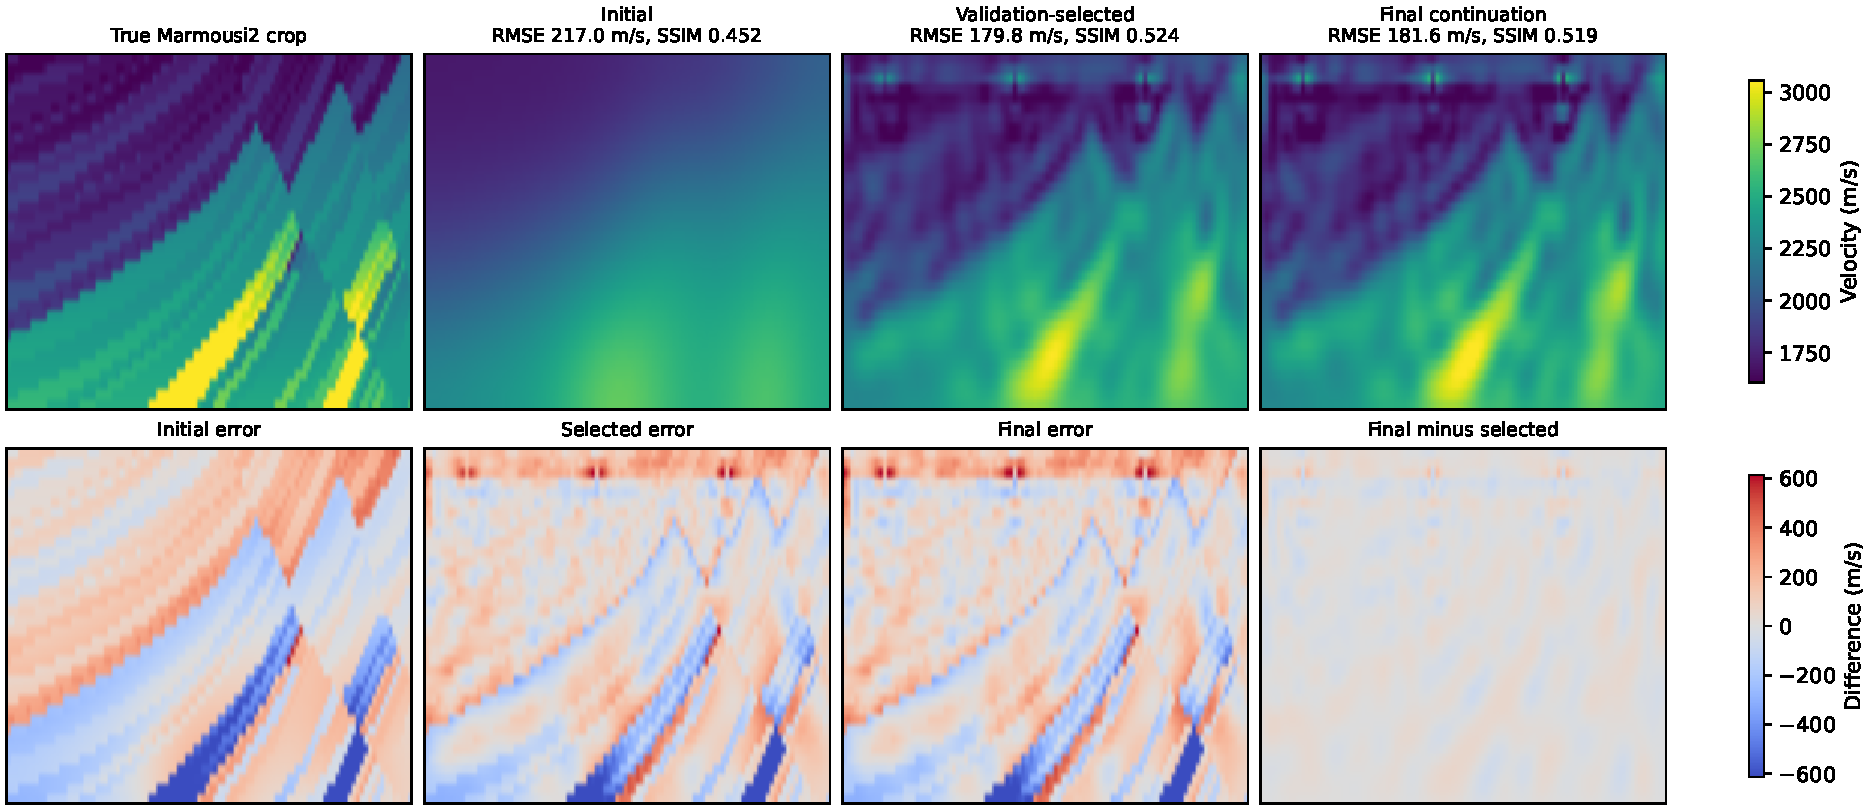
\includegraphics[width=0.98\textwidth]{fig_validation_primary_models.pdf}
  \caption{Actual reconstructed velocity models for the primary clean
  cross-grid experiment. The validation-selected and final continuation
  models are visually similar, but the error maps show that later
  continuation increases localized structural errors while reducing
  training-shot misfit.}
  \label{fig:primarymodels}
\end{figure*}

\subsection{Shot-Split Repetitions on the Primary Crop}
Table~\ref{tab:splits} summarizes three shot partitions on the primary
crop. In all three splits, validation-selected stopping improves RMSE,
SSIM, $R^2$, and edge correlation relative to final continuation.

\begin{table*}[t]
\centering
\caption{Held-out shot split repetitions on the primary crop. Each metric
is reported as validation-selected/final continuation.}
\label{tab:splits}
\begin{tabular}{lrrrrr}
\toprule
Split & Selected chunk & RMSE & SSIM & $R^2$ & Edge corr. \\
\midrule
Even-odd & 2 & 179.76 / 181.61 & 0.5241 / 0.5187 & 0.8133 / 0.8094 & 0.2648 / 0.2556 \\
Left-center & 4 & 184.40 / 185.48 & 0.5003 / 0.4945 & 0.8035 / 0.8012 & 0.1851 / 0.1703 \\
Outer-inner & 3 & 177.45 / 178.16 & 0.5208 / 0.5162 & 0.8181 / 0.8166 & 0.2404 / 0.2299 \\
\bottomrule
\end{tabular}
\end{table*}

Table~\ref{tab:splitsens} restates the same split repetitions as a
sensitivity summary in terms of improvement over final continuation. The
validation set size is fixed at three shots; this is therefore a
sensitivity check over held-out-shot placement rather than a full
cross-validation study. The selected checkpoint varies from chunks 2 to 4,
but all three split definitions retain positive gains in RMSE, SSIM, and
edge correlation.

\begin{table*}[t]
\centering
\caption{Validation-split sensitivity on the primary crop. Gains are
defined as final continuation minus validation-selected for RMSE, and
validation-selected minus final continuation for SSIM and edge
correlation.}
\label{tab:splitsens}
\begin{tabular}{lrrrr}
\toprule
Split & Selected chunk & RMSE gain (m/s) & SSIM gain & Edge-corr. gain \\
\midrule
Even-odd & 2 & 1.85 & 0.0054 & 0.0093 \\
Left-center & 4 & 1.08 & 0.0058 & 0.0149 \\
Outer-inner & 3 & 0.71 & 0.0046 & 0.0105 \\
Mean & 3.0 & 1.21 & 0.0053 & 0.0115 \\
\bottomrule
\end{tabular}
\end{table*}

\begin{figure*}[t]
  \centering
  
\includegraphics[width=0.95\textwidth]{fig_validation_random_splits.pdf}
  \caption{Primary-crop shot-split repetitions. Validation selection
  consistently avoids the final continuation degradation across the three
  tested shot partitions.}
  \label{fig:splits}
\end{figure*}

\begin{figure*}[t]
  \centering
  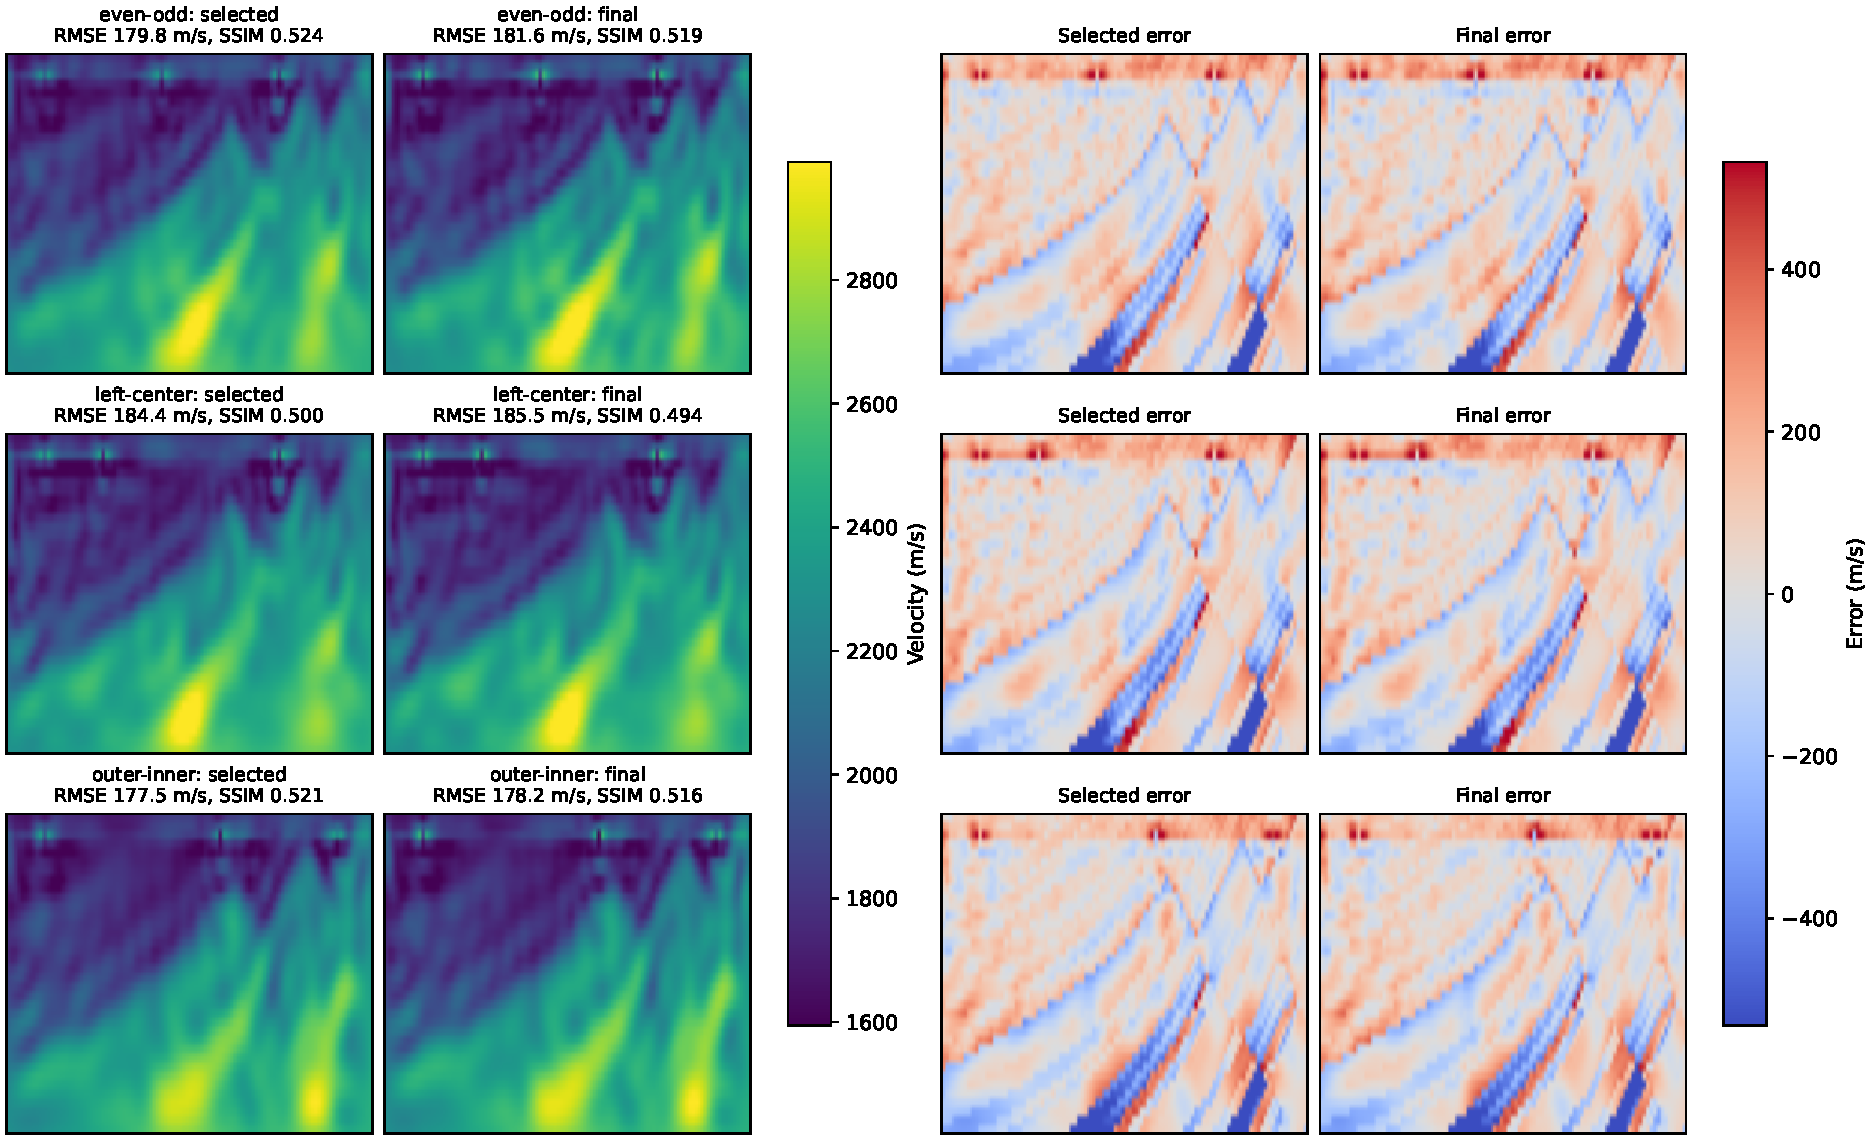
\includegraphics[width=0.98\textwidth]{fig_validation_split_models.pdf}
  \caption{Actual selected and final reconstructed models across the three
  primary-crop shot splits. Each row compares validation-selected and final
  continuation models and their corresponding errors against the true
  coarse Marmousi2 crop.}
  \label{fig:splitmodels}
\end{figure*}

\subsection{Noisy Cross-Grid Data}
Table~\ref{tab:noise} shows that the validation rule remains useful when
additive noise is applied after calibration. At both 20 dB and 10 dB, the
validation-selected checkpoint is chunk 2 and outperforms final
continuation in RMSE, SSIM, $R^2$, and edge correlation.

\begin{table*}[t]
\centering
\caption{Noisy cross-grid experiments on the primary crop. Metrics are
reported as validation-selected/final continuation.}
\label{tab:noise}
\begin{tabular}{rrrrrr}
\toprule
SNR (dB) & Selected chunk & Val. misfit & RMSE & SSIM & Edge corr. \\
\midrule
20 & 2 & 26588.77 / 27855.96 & 180.13 / 181.70 & 0.5229 / 0.5183 & 0.2598 / 0.2548 \\
10 & 2 & 83948.55 / 85300.74 & 180.30 / 182.55 & 0.5204 / 0.5141 & 0.2596 / 0.2506 \\
\bottomrule
\end{tabular}
\end{table*}

\begin{figure*}[t]
  \centering
  
\includegraphics[width=0.95\textwidth]{fig_validation_noisy.pdf}
  \caption{Noisy validation experiments. Held-out shot validation remains
  aligned with improved true-model metrics at both tested noise levels.}
  \label{fig:noise}
\end{figure*}

\begin{figure*}[t]
  \centering
  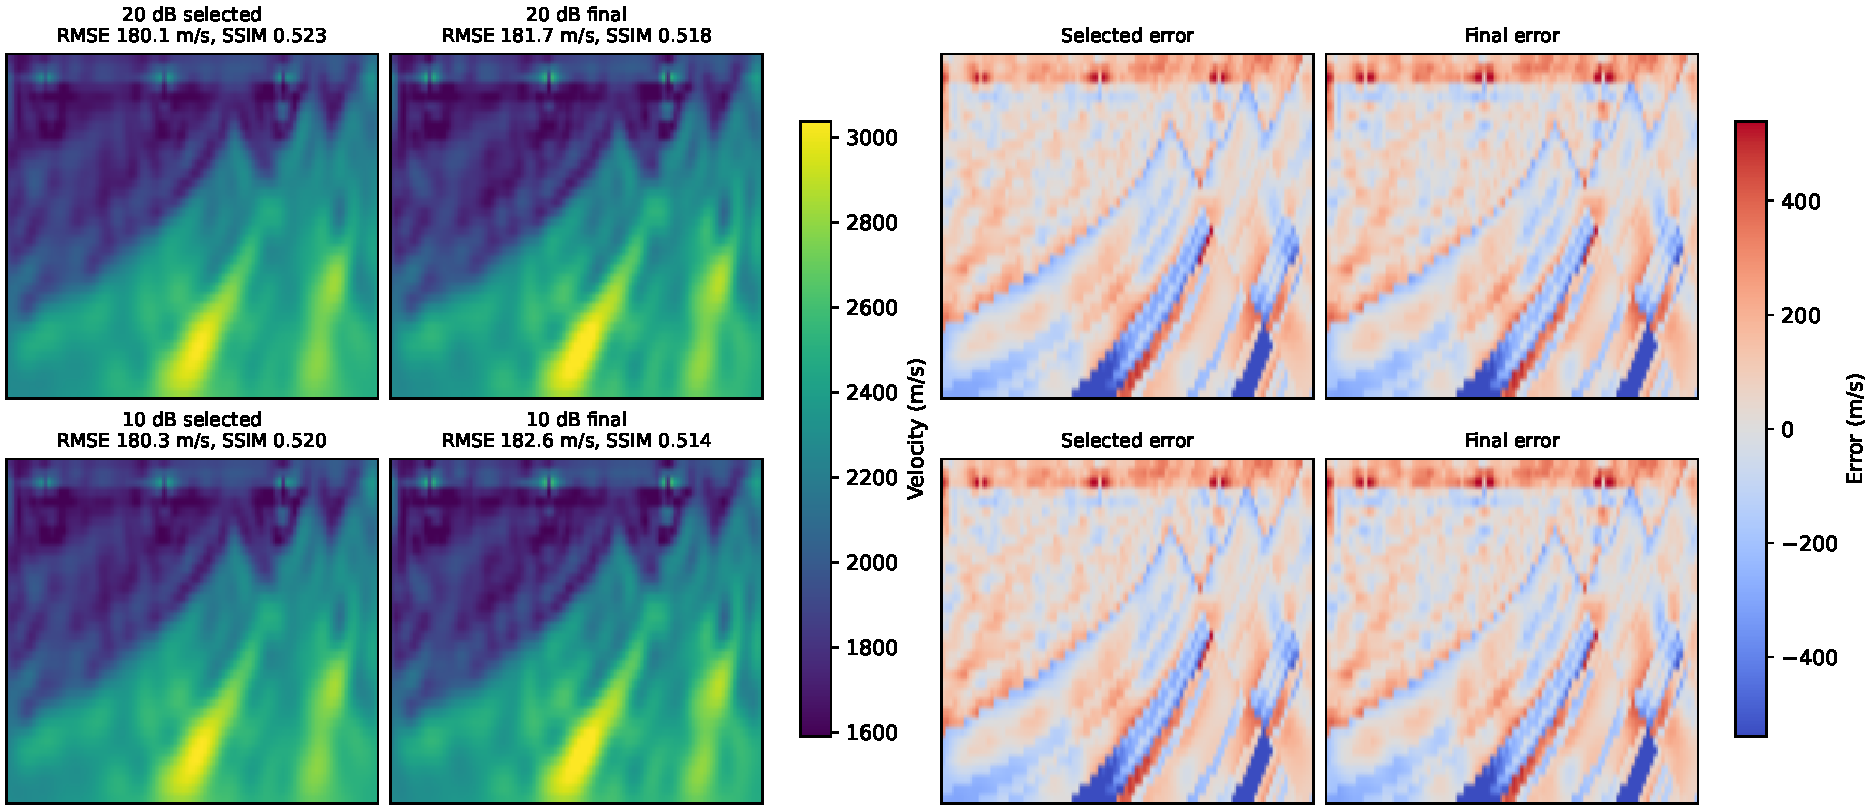
\includegraphics[width=0.98\textwidth]{fig_validation_noisy_models.pdf}
  \caption{Actual noisy-data reconstructions at 20 dB and 10 dB. The
  validation-selected models preserve slightly lower error than the final
  continuation models despite the additional data perturbation.}
  \label{fig:noisymodels}
\end{figure*}

\subsection{Second Crop and Longer Continuation}
The second crop is harder: the starting model has RMSE 320.83 m/s and
SSIM 0.3953 before inversion, compared with 216.99 m/s and 0.4517 on the
primary crop. Eight-chunk runs did not always exhibit overfitting by the
end of continuation, so we extended the second crop to 16 chunks. Results
are shown in Table~\ref{tab:cropb}. Validation selection improves the
final model in two of three splits. In the left-center split, validation
keeps improving through the final chunk, so the selected model is the
final model. This is a useful failure mode: the method does not force an
early stop when the held-out criterion does not indicate overfitting.

\begin{table*}[t]
\centering
\caption{Second-crop long continuation ($x_0=9500$ m, $z_0=900$ m,
$\sigma=8$, 16 chunks). Metrics are validation-selected/final
continuation.}
\label{tab:cropb}
\begin{tabular}{lrrrr}
\toprule
Split & Selected chunk & RMSE & SSIM & Edge corr. \\
\midrule
Even-odd & 14 & 248.27 / 249.21 & 0.5530 / 0.5518 & 0.2748 / 0.2707 \\
Left-center & 15 & 255.90 / 255.90 & 0.5391 / 0.5391 & 0.2836 / 0.2836 \\
Outer-inner & 14 & 264.97 / 266.78 & 0.5093 / 0.5078 & 0.2014 / 0.1962 \\
\bottomrule
\end{tabular}
\end{table*}

\begin{figure*}[t]
  \centering
  
\includegraphics[width=0.95\textwidth]{fig_validation_random_splits_cropB_long.pdf}
  \caption{Second-crop long-continuation results. The validation rule
  detects later overfitting in two splits and selects the final checkpoint
  when validation does not deteriorate.}
  \label{fig:cropb}
\end{figure*}

\begin{figure*}[t]
  \centering
  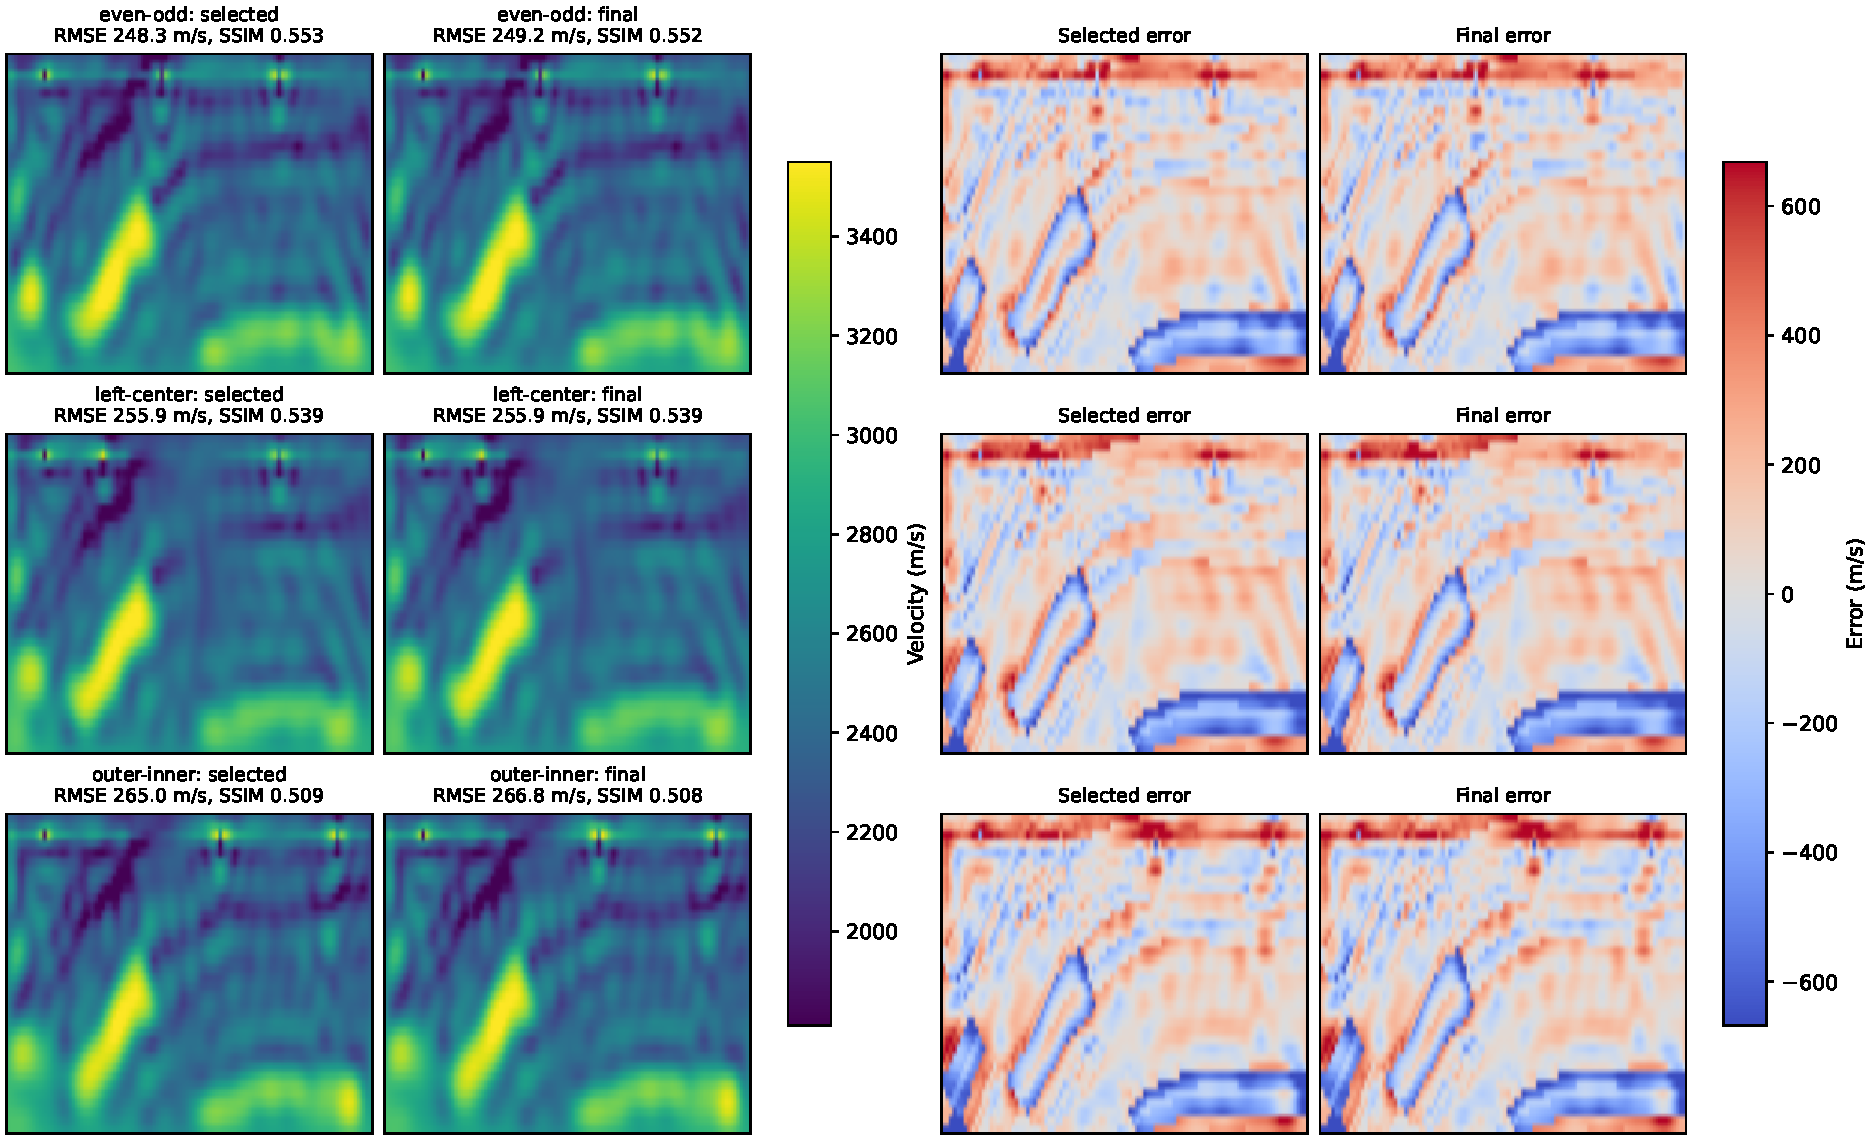
\includegraphics[width=0.98\textwidth]{fig_validation_cropB_models.pdf}
  \caption{Actual second-crop reconstructions for the long-continuation
  split repetitions. The effect is more limited than in the primary crop:
  two splits show validation-selected improvements, whereas the
  left-center split selects the final checkpoint because validation misfit
  does not deteriorate before the last chunk.}
  \label{fig:cropbmodels}
\end{figure*}

\subsection{Relation to Oracle Stopping}
Table~\ref{tab:oracle} compares validation-selected stopping with the
inaccessible oracle checkpoint. On the primary crop and noisy variants,
validation selection is close to the oracle RMSE checkpoint and often
exactly matches or nearly matches the oracle SSIM checkpoint. The second
crop has larger oracle gaps, especially in the outer-inner split, showing
that held-out validation is useful but not equivalent to knowing the true
model.

\begin{table*}[t]
\centering
\caption{Validation-selected stopping versus oracle stopping. RMSE gain is
final RMSE minus selected RMSE; RMSE gap is selected RMSE minus oracle-best
RMSE. SSIM gain and gap are defined analogously with higher SSIM better.}
\label{tab:oracle}
\begin{tabular}{lrrrr}
\toprule
Scenario & RMSE gain & RMSE gap & SSIM gain & SSIM gap \\
\midrule
Primary even-odd & 1.849 & 0.117 & 0.0054 & 0.0000 \\
Primary left-center & 1.078 & 0.436 & 0.0058 & 0.0040 \\
Primary outer-inner & 0.707 & 0.015 & 0.0046 & 0.0006 \\
20 dB noise & 1.565 & 0.443 & 0.0046 & 0.0000 \\
10 dB noise & 2.252 & 0.359 & 0.0062 & 0.0005 \\
Second crop even-odd & 0.943 & 2.616 & 0.0012 & 0.0060 \\
Second crop left-center & 0.000 & 0.958 & 0.0000 & 0.0000 \\
Second crop outer-inner & 1.801 & 8.103 & 0.0015 & 0.0084 \\
\bottomrule
\end{tabular}
\end{table*}

% =====================================================================
\section{Discussion}
% =====================================================================
\subsection{Why Held-Out Shots Matter}
Held-out receiver validation was also tested during method development,
but it was less reliable: receiver subsets share the same shot wavefields
and can reward models that fit acquisition-specific artifacts while
degrading true-model metrics. Held-out shots are a stricter validation
unit because source location changes the illuminated wavefield and the
path distribution. This makes the validation misfit more sensitive to
continuation overfitting under the cross-grid mismatch.

\subsection{What the Method Does and Does Not Solve}
The proposed rule is a stopping and model-selection procedure. It does
not change the acoustic physics, remove cycle skipping, or correct the
coarse-grid operator. Its value is operational: when training misfit keeps
falling after the recovered model begins to degrade, held-out shots
provide a measurable warning. The second crop demonstrates the limitation.
Validation stopping can avoid degradation when overfitting is visible in
held-out shots, but it cannot guarantee the oracle checkpoint for all
geological structures and shot partitions.

\subsection{Reproducibility and Practical Cost}
The validation rule adds forward-modeling cost because each checkpoint is
evaluated on held-out shots. In the present implementation, this cost is
small relative to broad parameter sweeps or neural reparameterization
experiments, and it does not require changing the adjoint implementation.
The experiments are fully script-based: data generation, calibration,
shot splits, optimization chunks, metric computation, and figures are
stored in the accompanying code and JSON summaries.

% =====================================================================
\section{Limitations}
% =====================================================================
This study is intentionally compact. The grid sizes are small enough for
rapid controlled experimentation, and only acoustic propagation is used.
The experiments do not include field data, elastic physics, attenuation,
anisotropy, source estimation, or realistic acquisition gaps. The
Marmousi2 ground truth is used only for evaluation, but the starting model
is still generated by smoothing the truth; future work should test
geologically independent initial models. Finally, validation selection
depends on whether held-out shots expose the same mismatch that causes
model degradation. The second-crop results show that this condition is not
automatic.

% =====================================================================
\section{Conclusion}
% =====================================================================
We presented a held-out shot validation rule for selecting FWI
continuation depth under controlled modeling mismatch. In a calibrated
Marmousi2 cross-grid setting, the rule identifies checkpoints that improve
true-model metrics relative to final training-driven continuation on the
primary crop, across three shot splits, and under 20 dB and 10 dB noise.
On a second crop the effect is partial: validation selection improves two
long-continuation splits and selects the final model when validation does
not indicate overfitting. The resulting contribution is not a new FWI
solver but a reproducible validation layer for deciding when continued
optimization has begun to fit the training acquisition more than the
underlying velocity model.

\section*{Computer Code Availability}
The source code and reproducibility materials used for this study are
available in a public GitHub repository at
\url{https://github.com/schumihuang/heldout-fwi-validation}. The repository
permits anonymous download and contains individual Python source files
rather than a compressed code archive, a README file with installation and
usage instructions, \texttt{requirements.txt}, \texttt{quick\_test.py},
the Marmousi2 data manifest and input file, saved JSON summaries, and
figure-generation scripts. The code is released under the MIT License. The
principal reproducibility entry points are
\texttt{code/run\_validation\_shot\_split\_crossgrid.py},
\texttt{code/run\_validation\_random\_splits.py},
\texttt{code/run\_validation\_noisy\_crossgrid.py}, and
\texttt{code/summarize\_validation\_oracle\_gap.py}.

\section*{Declaration of Competing Interest}
The authors declare that they have no known competing financial interests
or personal relationships that could have appeared to influence the work
reported in this paper.

\section*{Funding}
Funding information should be added by the authors before final
submission.

\section*{Author Contributions}
Author contribution details should be added by the authors before final
submission.

\bibliographystyle{plain}
\bibliography{refs_validation}
\end{document}
